\section{Die Formen des Universums}
Eine der spannendsten Fragen der Kosmologie ist eine ganz simple: Welche Form 
hat unser Universum?

Nach der Entdeckung und Messung der kosmischen Mikrowellenhintergrundstrahlung 
ist es uns möglich, diese Frage zu beantworten.
Die Frage nach der Form eines Körpers ist überraschend einfach durch die 
klassische Geometrie zu klären.
Grundsätzlich sind drei mögliche Formen denkbar:
\begin{itemize}
	\item Das Universum könnte positiv gekrümmt sein, wie eine Kugel.
	Zwei parallele Linien auf der Kugeloberfläche kreuzen sich und die 
	Winkelsumme eines Dreiecks ist grösser als 360 Grad (siehe Längengrade auf der Erdkugel).
	Beim Zurückblicken in der Zeit würde dies zu einem Vergrösserungseffekt führen,
	als würde man durch ein Fernrohr blicken.
	\item Das Universum könnte negativ gekrümmt sein, wie ein Sattel.
	Zwei parallele Linien weichen immer stärker voneinander ab und die 
	Winkelsumme eines Dreiecks ist kleiner als 360 Grad.
	Beim Zurückblicken in der Zeit würde dies zu einem Verkleinerungseffekt führen,
	als würde man auf der falschen Seite durch ein Fernrohr blicken.
	\item Das Universum könnte flach sein, wie ein Blatt Papier.
	Zwei parallele Linien berühren sich nie und die Winkelsumme eines Dreiecks 
	beträgt 360 Grad.
	Beim Zurückblicken, wären die Bilder so, wie wir sie es aufgrund der Berechnungen erwarten (wieso? --> erklären).
\end{itemize}
EINFÜGEN DER BILDER VOM SKRIPT

Diese Effekte würden sich auf die Bilder der kosmischen Mikrowellenhintergrundstrahlung
wie auf Abbildung \ref{fig:universe_shapes} auswirken.

\begin{figure}
	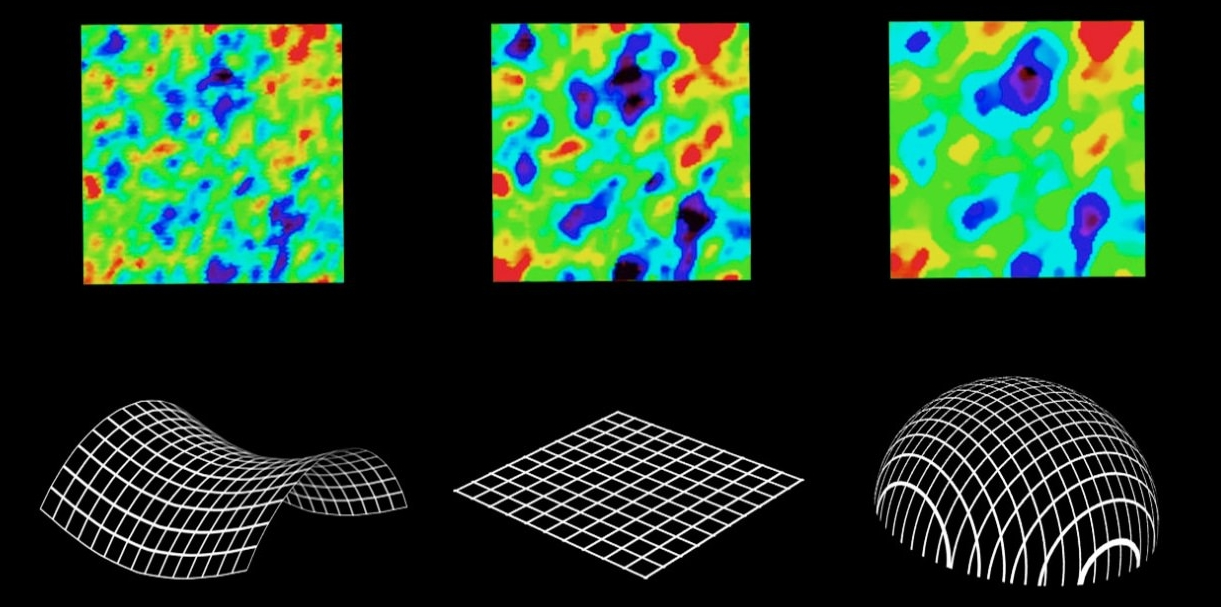
\includegraphics[width=\linewidth]{cmb/images/universe_shapes.jpg}
	\caption{Die drei möglichen Formen des Universums und die daraus 
		resultierenden Bilder des gleichen Ausschnitts der kosmischen
		Mikrowellenhintergrundstrahlung}
	\label{fig:universe_shapes}
\end{figure}